\chapter{Historical Background and Motivation}
\label{historical_background}

\section{Tricolor and its Inventor}

\textbf{Tricolor} is a board game invented in 1930 by \textbf{Maurice Kraitchik} (1882 – 1957) who was a Belgian mathematician, initially born in Russia, whose main interests were number theory and recreational mathematics \cite{rougetet_kraitchik}. He holds the patent for the game, which contains a photo of him (Figure~\ref{fig:maurice_photo}), an official certificate (Figure~\ref{fig:certificate_brevet}) and the rules of Tricolor written in French.

\begin{figure}[h]
    \centering
    % Horizontal box to keep text and image side by side
    \makebox[0pt][c]{%
        % Vertical text on the left
        \rotatebox{90}{\hspace{0pt}\tiny{AGR 1, Min. Just. Police des Étrangers Dossier individuel 1394574}}%
        \hspace{0em} % optional negative space to move text closer
        % The image
        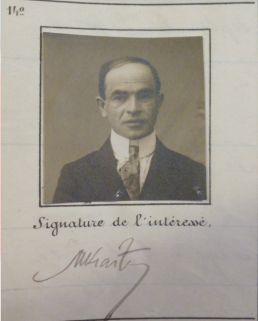
\includegraphics[scale=0.5]{historical_background/images/maurice_photo.png}%
    }
    \caption{Photo of Maurice Kraitchik from his patent for Tricolor}
    \label{fig:maurice_photo}
\end{figure}

\begin{figure}[h]
    \centering
    % Horizontal box to keep text and image side by side
    \makebox[0pt][c]{%
        % Vertical text on the left
        \rotatebox{90}{\hspace{0pt}\tiny{Kraïtchik, Maurice (1930) Tricolor. Brevet n°372711, Royaume de Belgique}}%
        \hspace{0em} % optional negative space to move text closer
        % The image
        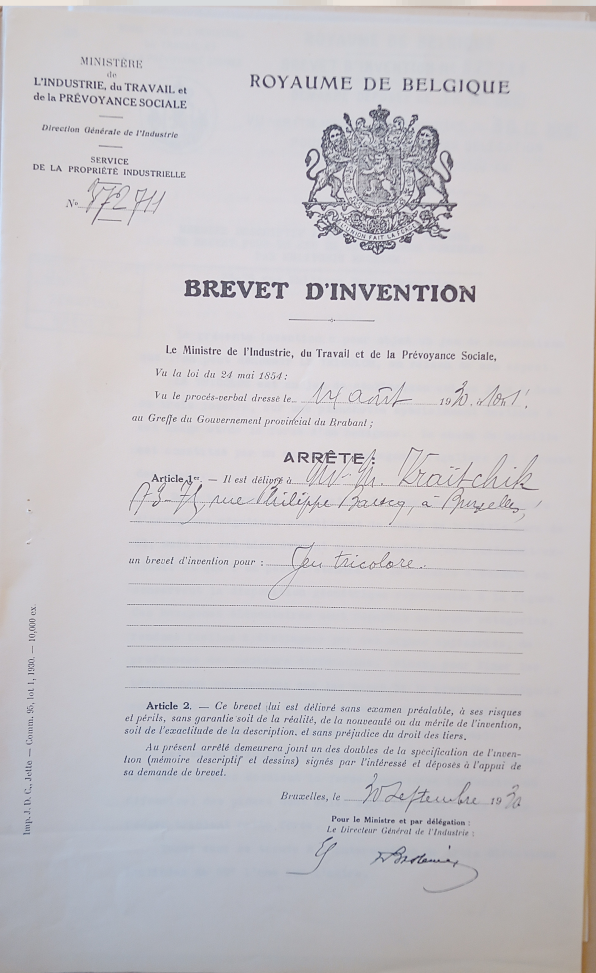
\includegraphics[scale=0.2]{historical_background/images/certificate_brevet.png}%
    }
    \caption{Photo of the official patent certificate for the invention of Tricolor}
    \label{fig:certificate_brevet}
\end{figure}

\section{Motivation}

\textbf{Tricolor} is the first board game in history to use a hexagonal tiling~\ref{fig:hex_tiling}. The unique gameplay features this structure enables, as well as its influence on later games adopting hexagonal tilings, constitute the main motivation for studying Tricolor.

The main objectives of this study on \textbf{Tricolor} are as follows:
\begin{enumerate}
\item To present the historical context of the game, including prior developments and subsequent research.
\item To analyze the game’s features and metrics, as well as its computational and strategic complexity.
\item To develop AI agents capable of playing the game at a high level.
\end{enumerate}

\section{Game Mechanics}

Tricolor is a complex combinatorial game due to the high number of possible moves at each turn. The main features that make the game unique are the hexagonal board tiling (such a tiling looks like the one in Figure~\ref{fig:hex_tiling}), the ability to stack pieces on top of each other, winning by capturing the opponent's pieces and the need to control the board in order gain an advantage. So far, Tricolor is known by historians as the first game in history to be using a hexagonal board tiling, which even today is quite a rare tiling used in games.

\begin{figure}[h]
    \centering
    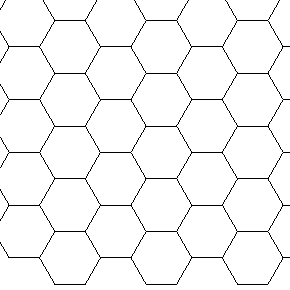
\includegraphics[scale=0.7]{historical_background/images/hex_tiling.pdf}
    \caption{Example of general hex tiling design}
    \label{fig:hex_tiling}
\end{figure}

\section{Similar previous Games}

The only game known by historians to be similar to Tricolor and invented before is \textbf{Laska} (also known as \textbf{Lasca}). Laska is a board game invented by the chess world champion and German mathematician Emanuel Lasker (1868–1941) in 1911 \cite{rougetet_sphinx}. The game has similar mechanics to Tricolor, such as being a combinatorial game, being able to stack pieces on top of each other by moving them around and controlling the board by blocking the opponent and capturing his pieces (see Figure~\ref{fig:Laska}).

AI techniques such as Monte Carlo Tree Search and Deep Neural Networks have already been investigated for playing Lasca, but they have been shown to perform poorly. This is partly due to the fact that Lasca allows pieces to be stacked on top of each other\footnote{as in Tricolor}, which increases the number of channels required in tensor-based game representations. Consequently, this also leads to a larger number of trainable parameters in the neural network architecture~\cite{ludii_and_polygames}.

As Maurice Kraitchik claims in the patent description, Tricolor was directly inspired from Laska.

\begin{figure}[h]
    \centering
    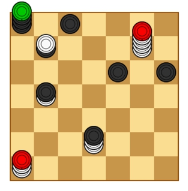
\includegraphics[scale=0.6]{historical_background/images/laska.png}
    \caption{Image with Laska board}
    \label{fig:Laska}
\end{figure}


\section{What was studied so far}

To date, there are no known papers or articles—whether physical or online—addressing the strategies or mathematical properties of Tricolor, apart from the book \textit{La mathématique des jeux ou récréations mathématiques} by Maurice Kraitchik (Stevens Frères, 1930). This work contains a wide range of mathematical problems of varying difficulty, as well as a chapter dedicated to Tricolor. In this chapter, the author introduces the rules of the game, defines a notation for possible moves, and presents two example games (see Figure~\ref{fig:games_examples}). He also discusses several endgame scenarios in which one player holds a slight material advantage and illustrates how the advantaged player can secure a win in the shortest possible way. While this analysis provides useful insight into certain strategic elements, it only covers a limited subset of the game’s possible positions. As a result, a more comprehensive study is still required to develop robust strategic theories for the game.

\begin{figure}[h]
    \centering
    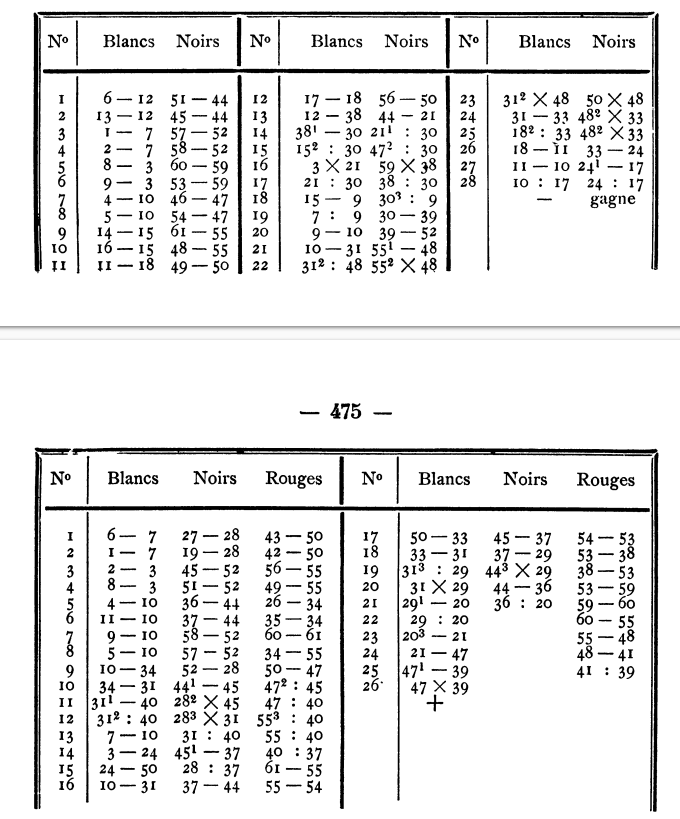
\includegraphics[scale=0.5]{historical_background/images/games_examples.png}
    \caption{Example of 2 possible games to be played}
    \label{fig:games_examples}
\end{figure}